\section{Résultats}

\paragraph*{Mesures}
L'approche critique a été réalisée en commencant à \(h_0 = 920.0 \pm 0.1\) mm. À chaque hauteur, le courant \(I\), ainsi que le nombre de neutrons \(n\) et temps \(t\) écoulé ont été mesurés. Le taux taux de compte \(C\) est alors déterminé avec \(C = n/t\). Les hauteurs où les mesures ont été réalisées ainsi que les valeurs mesurées sont reportées dans le \autoref{tab:mesures}.

\begin{table}[h]
    \centering
    \begin{tabular}{ |c||c|c|c|c|c| }
        \hline
        h [mm] & I [nA] & n & t [s] & C [\si{\per\second}] \\
        \hline\hline
        \(920.0 \pm 0.1\) & \(0.30 \pm 0.02\) & \(10006 \pm 100\) & \(391.6 \pm 0.1\) & \(25.5 \pm 0.3\) \\
        \(930.0 \pm 0.1\) & \(0.42 \pm 0.02\) & \(10010 \pm 100\) & \(279.8 \pm 0.1\) & \(35.7 \pm 0.4\) \\
        \(938.3 \pm 0.1\) & \(0.67 \pm 0.02\) & \(10002 \pm 100\) & \(188.2 \pm 0.1\) & \(53.1 \pm 0.5\) \\
        \(943.1 \pm 0.1\) & \(1.1 \pm 0.2\) & \(10015 \pm 100\) & \(126.9 \pm 0.1\) & \(78.9 \pm 0.8\) \\
        \hline
    \end{tabular}
    \caption{Hauteur d'eau dans le réacteur, courant, compte, temps de compte et taux de compte obtenus}
    \label{tab:mesures}
\end{table}

\paragraph{Estimations avec courant}
En accord avec la théorie, la hauteur critique est proportionnelle à l'inverse du courant. En utilisant la méthode décrite dans la démarche expérimentale, la hauteur critique \(h_c\) a été déterminée. Une estimation sur l'erreur est obtenue de manière graphique, comme décrit dans \autoref{sec:erreurs}. Les résultats sont présentés dans \autoref{fig:hc_intensite}. Une hauteur critique entre 950 et 955 a alors été trouvé. Expérimentalement, l'opérateur a montré que la hauteur critique était \(h_c = 952.2 \pm 0.1\) mm.

\begin{figure}[H]
    \centering
    \begin{subfigure}{0.48\linewidth}
        \centering
        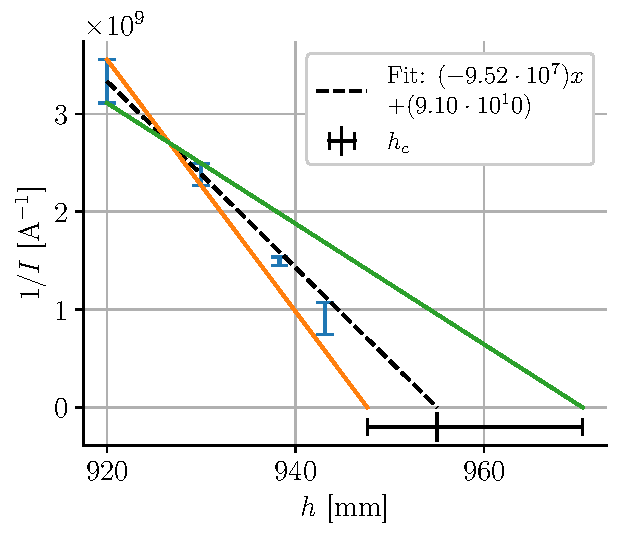
\includegraphics[width=\linewidth]{figures/h_I_pair12.pdf}
        \caption{}
        \label{fig:hc_I_12}
    \end{subfigure}
    \begin{subfigure}{0.48\linewidth}
        \centering
        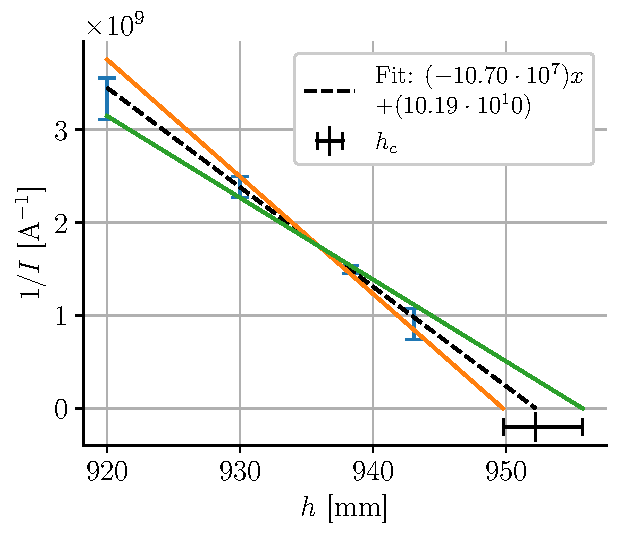
\includegraphics[width=\linewidth]{figures/h_I_pair23.pdf}
        \caption{}
        \label{fig:hc_I_23}
    \end{subfigure}
    \begin{subfigure}{0.48\linewidth}
        \centering
        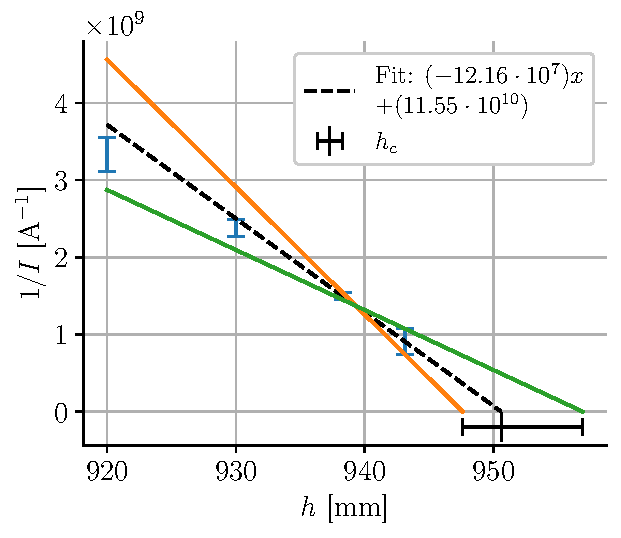
\includegraphics[width=\linewidth]{figures/h_I_pair34.pdf}
        \caption{}
        \label{fig:hc_I_34}
    \end{subfigure}
    \begin{subfigure}{0.48\linewidth}
        \centering
        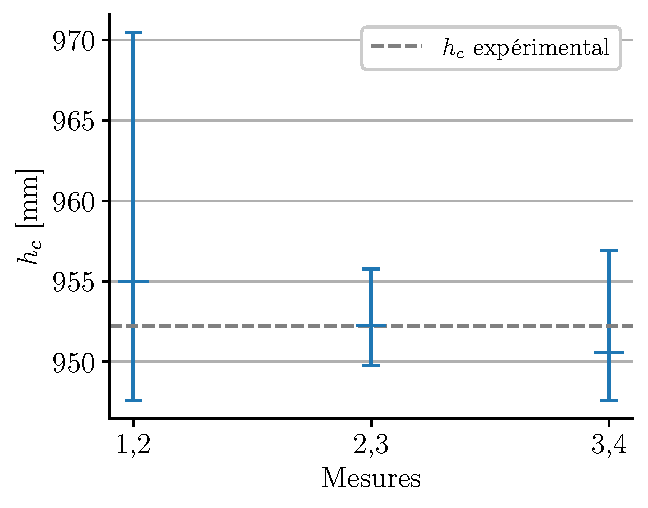
\includegraphics[width=\linewidth]{figures/hc_results_I.pdf}
        \caption{}
        \label{fig:hc_I}
    \end{subfigure}
    \caption{Estimations de \(h_c\) avec une régression linéaire en utilisant les mesures (a) 1 et 2, (b) 2 et 3, (c) 3 et 4. En (d) les hauteurs critiques \(h_c\) trouvées, ainsi que l'estimation de l'erreur sur la valeur trouvée.}
    \label{fig:hc_intensite}
\end{figure}

\paragraph*{Estimations avec taux de compte}
feur